%!TEX root = thesis.tex
\chapter{Cryptographic Primitives}
Secure Compuation (SC) is the study of computing functions in a secure fashion. 
SC can be split into two cases: cases where there are two parties involved, referred to as two-party computation (2PC), and cases where there are three or more parties, referred to as multiparty computation (MPC).
This thesis will focus primarily on 2PC protocols, but many of the methods are applicable to MPC as well.

2PC protocols are complex cryptographic protocols that rely on a number of cryptographic primitives.
In order to understand 2PC, it is not crucial to understand how the cryptographic primitives work, but it is important to understand their inputs, outputs and security guarantees. 
This first chapter will give an overview of the cryptographic primitives used in 2PC protocols.

\section{A Brief Introduction to Cryptography} 
What does it mean for a cryptographic scheme to be secure? 
THe goal of this section is to explain cryptographic security, starting at an intuitive level and moving outward. 
We do not present cryptographic security in a comprehensive fashion; rather we explain security with the goal of explaining 2PC protocols and their security.
For more information on cryptographic security, we encourage the reader to peruse \cite{textbook}. 

\al{this paragraph is weak, but on the right track}
Cryptographic schemes are premised on problems. 
At the simples level, as long as the underlying problem is difficult to solve, then the cryptographic scheme is secure.
One can imagine that there are two types of problems.
The first type of problem is solvable if one has access to infinite computational time and space\footnote{Space, in computer science, refers to computer memory}. 
The second type of problem, a subset of the former, is solvable with reasonable computational time and space. 
Reasonable time and space could mean various things - a few hours, a few lifetimes, a few computers or a few universes - depending on the context. 
The reason that I make the distinction between problems that are solved with reasonable resources and those that aren't, is because these are the types of problems that cryptography is concered with. 
Cryptographers are not concerned if you can solve a problem in a couple hundred years, because that's not relevent to the security of today. 

Cryptographers need to be precise about how difficult the problem underlying a cryptograpic scheme is, and this is acheived in two ways. 
The first way is to restrict what algorithms trying to solve the problem to polynomial-time algorithms.
A polynomial-time algorithm requires $p(n)$ steps, hwere $p$ is some polynomial and $n$ is the size of the input to the problem. 
Often, polynomial-time algorithms are called \textit{efficient} because they generally not \textit{brute-forcing} a solution to the problem; instead, they use some trick or shortcut to efficiently find an answer.

The second adaptation that cryptographers make to problems is tuning the difficulty of the problem. 
Consider that the problem underlying a cryptographic scheme is finding the factors of $N$, where $N$ is some known large number.
This problem may be made easier or harder by changining how large $N$ is. 
In fact, if $N < 10,000$, then your laptop can find the answer in mere seconds. 
If $N$ is really large, finding the factors using the best known current methods could take decades. 

\al{get these to flow better}
If a cryptographic scheme is premised on factoring a large number, and it turns out that there is some efficient, reasonably fast algorithm for factoring large numbers, then we would say that the cryptographic scheme is broken. 
More formally, a cryptographic scheme is broken if the problem underlying it may be solved efficiently.

To formalize the idea of scalable security, we introduce the \textit{security parameter} and denote the security parameter as $\lambda$. 
The security parameter corresonds to the difficulty of the underlying problem of a cryptgraphic scheme. 
When the security parameter increases, the cryptographic scheme becomes harder to break.



\label{sctn:computational-indistinguishability}
We formally define computational indistinguishability as follows.

\begin{definition}
\label{defn:computational-indistinguishability}
\al{Adam noted that a might be redundant, and the counting parameter might be confusing}
Let $\mathcal{X} = \{X(n,a)\}_{n \in \NN, a \in \{0,1\}^*}$ and $\mathcal{Y} = \{Y(n,a)\}_{n \in \NN, a \in \{0,1\}^*}$ be distribution ensembles.
$\mathcal{X}$ and $\mathcal{Y}$ are computationally indistinguishable, denoted $\mathcal{X} \compindist \mathcal{Y}$, if and only if for all non-uniform polynomial-time distinguisher $D$, there exists a function $\mu(\cdot)$ that is negligible in $n$, such that for all $a \in \{0,1\}^*$, 
\begin{equation}
    |Pr[D(X(n,a)) = 1] - Pr[D(Y(n,a)) = 1]| < \mu(n)
\end{equation}
\cite{lindell2009secure}.
\end{definition}

\begin{definition}
\label{defn:negible}
A function $\mu : \NN \to \RR$ is negligible if for all positive polynomial $p(\cdot)$, there exists positive integer $N_p$ such that for all $x > N_p$, 
\begin{equation}
    |\mu(x)| < \frac{1}{p(x)}.
\end{equation}
\cite{goldreich}
\end{definition}

\section{Encryption}
\al{add in from google drive}
\begin{equation}
    \label{eqn:encryption}
    \begin{split}
        \Enc_k (pt) & = ct  \\
        \Dec_k(pt) = \EncInv_k(ct) & = pt
    \end{split}
\end{equation}
where $pt$ is the original message or the \emph{plaintext}, $ct$ is the encrypted message or the \emph{ciphertext}, and $k$ is the secret key.
For the algorithm to be effective, the secret key $k$ must be randomly sampled from $\{0,1\}^\lambda$, where $\lambda$ is the security parameter of our protocol.\footnote{The notion of randomness in cryptography is precisely defined, and in cases where $\lambda$ is large, it is sufficient for $k$ to be pseudorandom. Pseudorandomness is also precisely defined.}
\al{does footnote go before or after period? ShouldI have footnotes?}
If  $\lambda$ is increased, thereby increasing the size of the key, then the encryption algorithm becomes harder to break.
We will not go into details about how encryption algorithms are instantiated; we will merely treat them as algorithms which we can use at our leisure.

\begin{definition}
\al{Get crypto book and finish this}
We say that an encryption scheme is secure if:\footnote{Specifically, this is the definition of a chosen-plaintext-attack secure encryption scheme. There exists weaker and stronger definitions of security, but chosen-plaintext-attack security is frequently used for 2PC}

Define the following game:
What are the inputs?
\begin{enumerate}
\item Adversary picks two messages $m_0$ and $m_1$, and gives $m_0$ and $m_1$ to the sender. 
\item The sender samples $k \gets \{0,1\}^{\lambda}$ and $b \gets \{0,1\}$. The sender gives $m_b$ to the adversary. 
\item The adversary may spend a polynomial amount of time doing computation. Eventually, the output $b'$, their guess as to which message they received.
\end{enumerate}
\end{definition}
% END WORK HERE

It is useful for 2PC to define a specific type of symmetric-key encryption algorithm called a \textit{dual-key cipher} (DKC) \cite{bellare2012foundations}.
A DKC requires two keys to encrypt and decrypt the message, in contrast to classic encryption which only requires one.
It is easy to instantiate a DKC if one has a secure encryption scheme: let $k_0$ and $k_1$ be two keys and instantiate the DKC as follows:
\begin{equation}
    \begin{split}
        \EncDKC_{k_0, k_1}(pt) = \Enc_{k_1} ( \Enc_{k_0} ( pt )) \\
        \EncDKCInv_{k_0, k_1}(ct) = \EncInv_{k_0} ( \EncInv_{k_1} ( ct )) 
    \end{split}
\end{equation}
This construction of a DKC is slow, and there are many faster methods for instantiating DKCS.
For more information, see \cite{bellare2012foundations}.

\section{Boolean Circuit} 
A function in a 2PC protocol is represented as a boolean circuit.
A boolean circuit takes as input $x \in \{0,1\}^n$, performs a series of small operations on the inputs, and outputs $y \in \{0,1\}^m$.  
You may have encountered circuits and logical operators in another context, where the inputs and outputs were True and False.
For our usage, True will correspond to the value $1$, and False will corresond to the value $0$. 

The small operations done inside of a circuit are performed by a \emph{gate}.
A gate is composed of three wires: two input wires and one output wire, where a \emph{wire} can have a value either $0$ or $1$.
A gate performs a simpler operation on the two inputs, resulting in a single output bit.
Table \ref{tab:xor} gives the mapping of an XOR gate.

\begin{table}[h]
\label{tab:xor}
\centering
\begin{tabular}{ | l | c || r |}
\hline
x & y & xor(x,y) \\ \hline
1 & 1 & 0 \\ \hline
1 & 0 & 1 \\ \hline
0 & 1 & 1 \\ \hline
0 & 0 & 0 \\ \hline
\end{tabular}
\caption{The mapping of an XOR gate.}
\end{table}

A circuit is a combination of gates that are stringed together.
It turns out that circuits are quite powerful: in fact, a circuit composed only of AND gates, XOR gates and NOT gates can compute any function or algorithm \cite{Goldreich}.
In other words, if there's some algorithm that can do it, then there is some circuit that can do it as well.
Figure \ref{fig:less_than_circuit} shows the circuit representation of the less than function, $f$ as specified in equation \ref{eqn:less_than}.

\begin{figure}[h]
    \centering
    \includegraphics[scale=0.75]{images/drawing.png}
    \label{fig:less_than_circuit}
    \caption{A circuit that computes the less or equal to function, equivalent to the less than function for input of two one-bit values.\al{define symbols and google circuit diagrams latex / tree diagrams}}
\end{figure}

\begin{table}[h]
\label{tab:less_than}
\centering
\begin{tabular}{ | l | c || r |}
\hline
x & y & $x < y$ \\ \hline
0 & 0 & 0 \\ \hline
0 & 1 & 1 \\ \hline
1 & 0 & 0 \\ \hline
1 & 1 & 0 \\ \hline
\end{tabular}
\caption{The truth table of the less than circuit.}
\end{table}

\section{Oblivious Transfer}
\al{more sources here - get from CompGC paper}
\al{Give a nice metaphor of using OT - what happens. Don't need to give the protocol}
Oblivious Transfer (OT) is a two-party protocol where one party (sender) has two inputs, $m_0$ and $m_1$, and the other party (receiver) has a bit $b \in \{0,1\}$. 
OT enables the receiver to acquire $m_b$ from the sender without revealing which message is received, i.e., the value of $b$.
Moreover, the receiver learns nothing about the message that isn't received, i.e. anything about $m_{1-b}$.

The protocol relies on the DDH assumption.\footnote{The Decisional Diffie-Hellman (DDH) assumption is a computational hardness assumption involving discrete logarithms in cyclic groups. For more information, see \cite{Boneh1998}.}


